\documentclass[12pt]{article}
\usepackage[margin=1in]{geometry}
\usepackage{amsmath,amssymb,graphicx,booktabs,hyperref,caption,placeins}
\captionsetup{font=small}
\setlength{\parskip}{4pt}
\renewcommand{\topfraction}{0.9}\renewcommand{\bottomfraction}{0.8}\renewcommand{\textfraction}{0.08}\renewcommand{\floatpagefraction}{0.85}
\setcounter{topnumber}{3}\setcounter{totalnumber}{4}
\title{Do Faster Optimizer Kernels Reduce End-to-End Training Time?\\[2pt]\large EECS 182 Final Report (V1)}
\author{Ethan Liu \and Justin Kim \and Dev Patel \and Ahilan Karuppusami}
\date{November 23, 2026}
\begin{document}
\maketitle

\begin{abstract}
The modded-nanoGPT speedrun is a public contest to train a small GPT-style language model to a validation loss of 3.28 on the FineWeb text dataset in the shortest time on eight H100 GPUs, and the record submission, ANVIL2, does so in about 40 seconds. At every training step its optimizer makes each weight-matrix update approximately orthogonal (all singular values near one) by applying six polynomial maps, each of which requires several matrix products, and we measured how much of the run this matrix work accounts for and whether computing it faster shortens the run. An ablation, which is a run that skips the maps and is used only for timing, shortens the 1193 timed steps by $0.26$\,s of a $40.6$\,s run ($0.6\%$, four seeds), which is an estimate of the upper bound on the saving from any faster implementation of the maps. An isolated benchmark measures $0.59$\,ms of matrix work per step and the ablation removes $0.22$\,ms per step, and in the benchmark the time of a matrix product at these sizes falls more slowly than its arithmetic; from these comparisons we infer that part of the work overlaps other GPU activity and that GPU kernels (the functions that run on the GPU) may have a fixed cost per operation. As a test case we implemented an evaluation order that does most of the work on the small Gram matrix $X^\top X$ instead of the large matrix $X$, which is described in an appendix of the Polar Express paper and developed further as Gram Newton--Schulz; on the largest group of weight matrices it is $1.30\times$ faster on the matrix sequence and $1.08\times$ faster on the full update at the record's numerical accuracy, and it shortens the timed steps by $0.08$\,s ($0.2\%$, five paired seeds), while the whole-run difference of $0.05$\,s is not significant. This agrees with the absence of a runtime benefit that the Polar Express authors report at small scale.
\end{abstract}

\section{Introduction and background}
Matrix-aware optimizers change the geometry of a weight update as well as its size. Shampoo~\cite{shampoo} preconditions each weight tensor with per-dimension statistics, and Anil et al.~\cite{anil} make this practical at scale. SOAP~\cite{soap} runs Adam in Shampoo's eigenbasis. Muon~\cite{muonblog}, studied at scale by Liu et al.~\cite{muon}, takes the momentum matrix $X$ (a running average of the gradients of one weight matrix), with singular value decomposition $X=U\Sigma V^\top$, and replaces it with an approximation of $UV^\top$. The matrix $UV^\top$ is the polar factor of $X$. It has the singular vectors of $X$ and all singular values equal to one, and replacing $X$ with it is called orthogonalization. Muon computes the approximation with a Newton--Schulz iteration, which applies an odd polynomial to $X$ several times and needs only matrix products. Polar Express~\cite{polar} tunes a separate polynomial for each round of that iteration. Other work reduces the cost of the orthogonalization by reusing results from earlier optimizer steps. CacheMuon~\cite{cachemuon} reuses information from previous steps to approximate the polar factor at the current step, and Transport Muon~\cite{transportmuon} keeps the previous polar factor, recomputes it in full every several steps and applies a small correction in between. We did not test these methods. Wen et al.~\cite{fantastic} show that claimed optimizer gains shrink under fair, well-tuned comparisons. For that reason we compare at fixed validation quality and report variance.

These optimizers use more computation per step in order to train in fewer steps. Whether the added computation affects wall-clock time depends on the rest of the training system. We study this in ANVIL2~\cite{anvil2}, the submission that holds the record in the modded-nanoGPT speedrun~\cite{speedrun}, and we refer to it as the record. Its forward and backward passes already use FP8 (8-bit floating-point) arithmetic~\cite{fp8}, FlashAttention-3~\cite{fa3}, custom Triton kernels~\cite{triton} and CUDA graphs. A kernel is a function that runs on the GPU, and Triton is a language and compiler for writing kernels from Python. A CUDA graph is a recorded sequence of kernel launches that is replayed as one unit. The optimizer could therefore be a visible share of the remaining time.

\paragraph{Setting.} The speedrun asks for the fastest training of a language model to a cross-entropy loss of at most 3.28 on the FineWeb validation set with eight NVIDIA H100 GPUs. The record applies its optimizer, ANVIL, to the projection matrices and applies Adam to the other parameters (embeddings, scalars and gate weights). According to the record's code, ANVIL differs from Muon in the following ways: it keeps two momentum averages for each matrix, one fast and one slow, and blends them after a fixed step; it replaces the Newton--Schulz iteration with six quintic (degree-five) polynomial maps that each have their own coefficients; and it rescales the update with a running variance estimate and gates weight decay on the sign of the slow average. A run has 1194 steps in five schedule stages, numbered 0 to 4. The stages differ in batch size (in the ratio 8:16:24:20:8) and in maximum document length (896, 2048 and then 3072 tokens), so the time of a step depends on the stage. The weight matrices have the same sizes in every stage, so the optimizer's matrix work per step does not change.

\paragraph{Questions.} (Q1) How much does ANVIL's matrix computation contribute to step latency, the wall-clock time of one training step? (Q2) Which of its operations can be accelerated without changing the update rule? (Q3) How much of that carries through to the time needed to reach the validation target?

\paragraph{Hypothesis.} The change we test is the Gram-space evaluation order, which computes the same maps with fewer products on the large matrix (Section~\ref{sec:method}). Amsel et al.~\cite{polar} report no runtime benefit from it at small scale (Muon on a GPT-Small model). The question here is whether this also holds in a more heavily optimized trainer, where the rest of the step is cheaper, and what bounds the gain. The hypothesis under test was that the matrix work is a few percent of the step, so that a faster implementation gives a measurable end-to-end gain.

\section{The optimizer's matrix work}
For each weight matrix, ANVIL forms a momentum matrix $X$ in bfloat16, a 16-bit floating-point format with about eight significant bits. It scales $X$ so that all singular values are below one, and applies six maps
\begin{equation}
A = X^\top X,\qquad X \leftarrow X\,(aI + bA + cA^2),
\end{equation}
each with its own coefficients $(a,b,c)$. The matrix $A=X^\top X$ is the Gram matrix of $X$. It is symmetric, and for a tall $X$ it is smaller than $X$. We use the word map for one application of this formula, as the record's code does. A map corresponds to one round of the Newton--Schulz iteration. In the basis of the singular value decomposition, a map sends every singular value $\sigma$ to $a\sigma+b\sigma^3+c\sigma^5$ and leaves the singular vectors unchanged. The six maps together send singular values above about $0.01$ to about $1$ (Figure~\ref{fig:maps}); a singular value of $0.001$ ends at $0.58$. The result is therefore an approximation of the polar factor.

\begin{figure}[!htb]\centering
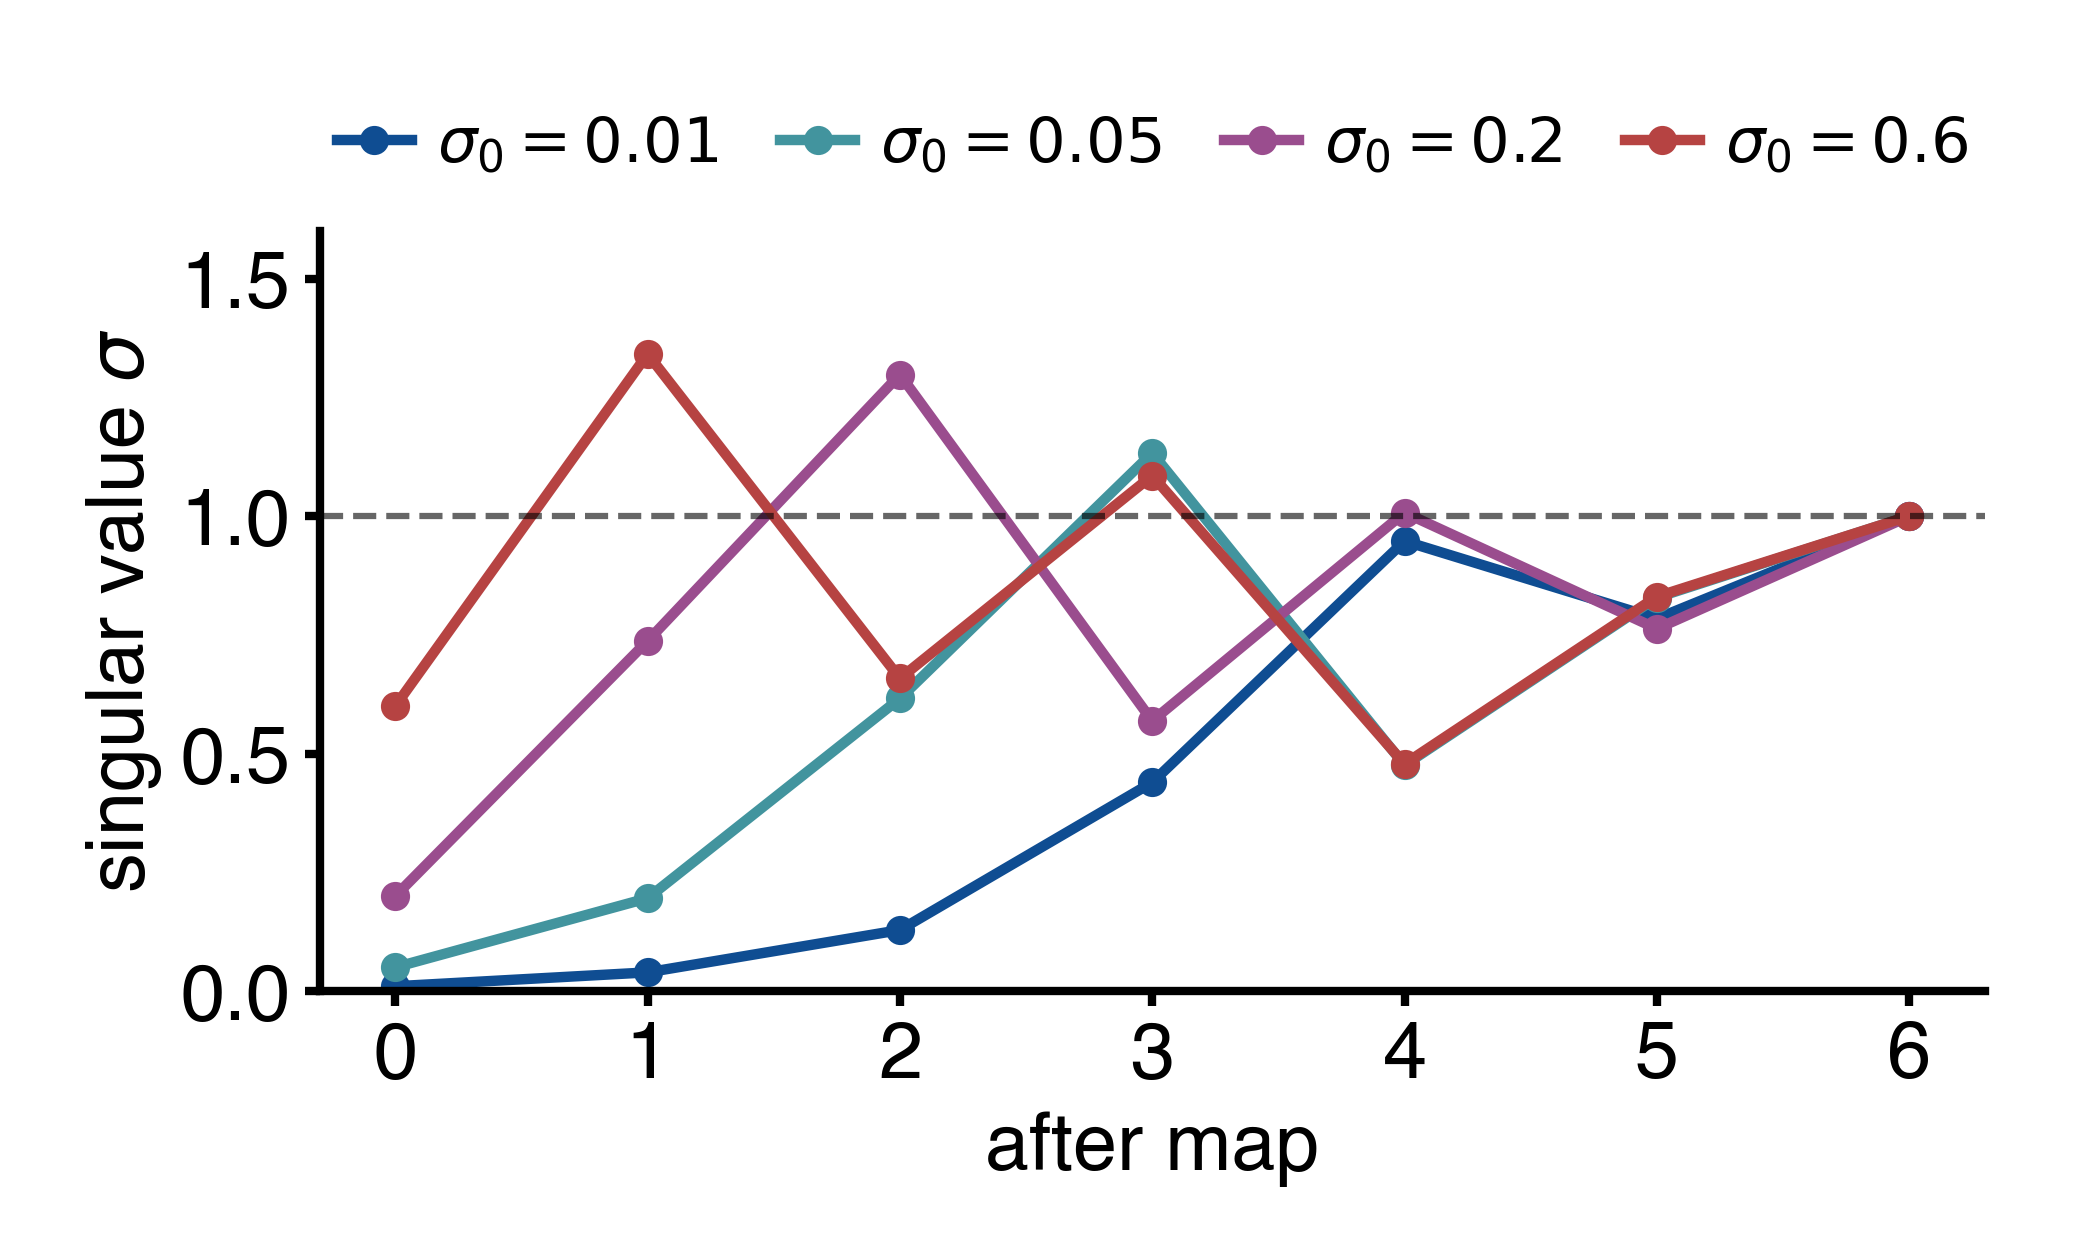
\includegraphics[width=0.55\linewidth]{fig_maps.png}
\caption{Four singular values through ANVIL's six maps, one line per starting value. Intermediate values overshoot 1 and return, and only the last map's output must be near 1.}\label{fig:maps}
\end{figure}

Matrices of the same shape are stacked into a weight group, which the code calls a bank, and one batched operation processes a whole group. Each GPU holds three groups: six matrices of size $256\times768$, two of size $768\times768$, and three of size $2816\times768$ (the MLP weights). For the MLP group, one map consists of a Gram matrix of the large matrix, a $768\times768$ polynomial, and a product with the large matrix. Six maps therefore make twelve passes over the large matrix. The record already computes symmetric products as half-products. A half-product is a product whose result is known to be symmetric, so that only the entries on one side of the diagonal are computed and the others are copied (mirrored) from them. The record also batches each group and replays the sequence of operations as one CUDA graph.

\section{Method}\label{sec:method}
\paragraph{Gram-space evaluation (Q2).} Write a map as $X\leftarrow XP$ with $P=aI+bA+cA^2$. Because $P$ is a polynomial in the symmetric matrix $A$, the Gram matrix for the next map is
\begin{equation}
(XP)^\top(XP) = P\,A\,P,
\end{equation}
which does not involve $X$. Two consecutive maps can therefore be evaluated on $768\times768$ matrices only: compute $A$, form $P_1$, compute $A'=P_1AP_1$, form $P_2$, and apply $Q=P_1P_2$ to $X$ once. For each pair of maps, this replaces two Gram matrix computations and two large products with one of each, plus three small products. We call this the Gram-space evaluation order. The update rule is unchanged, and in float64 arithmetic the two evaluation orders agree to rounding error (a check is in the repository's tests).

\paragraph{Origin of the method.} This evaluation order is not new. Amsel et al.~\cite{polar} give it in an appendix (``Fast Polynomial Iteration for Rectangular Matrices''), together with restarting from $X$ every few maps to control round-off in bfloat16. A restart means applying the accumulated product $Q$ to $X$ and computing the Gram matrix again from the new $X$. They also tried the method in Muon on a GPT-Small model, and they report a negligible change in loss, nearly identical runtimes, and that the FLOP savings were not beneficial at that scale. Zhang et al.~\cite{gramns} develop the same idea further as ``Gram Newton--Schulz''. They restart after two iterations for half-precision stability, use symmetric matrix-multiply kernels for the Gram-side products, and release code. They report 40--50\% less time in the orthogonalization step on large models, where that step is 2--17\% of wall-clock time. Our implementation makes the same choices (a restart every two maps and a symmetric kernel for the small products). Our implementation predates our reading of that work (the commit dates are in the repository), and we do not claim the method. We tested it in a more heavily optimized trainer, and we measured three quantities that bear on the size of the saving: how much optimizer time exists, how much of it is exposed, and how kernel time scales at these sizes.

\paragraph{The kernel.} Because the small operands are symmetric and commute, their product is symmetric, so it can be computed as a half-product. The Triton kernel that does this is adapted from the record's existing half-product kernel (\texttt{ba\_plus\_cAA}), with the second factor read from a second matrix. The same operation already exists in the symmetric matrix-multiply kernel that Zhang et al.~\cite{gramns} use for these products, so ours is a port of that operation to the record's kernel framework and is not a new kernel design. We call the resulting implementation of the Gram-space order \texttt{gram222s}. In the rest of this report, ``the kernel'' means \texttt{gram222s} as a whole, and ``a GPU kernel'' means a single GPU function.

\paragraph{Number of maps per restart.} The Gram matrix is stored in bfloat16. Its eigenvalues are $\sigma^2$, so small singular values may fall below its rounding error. Zhang et al.~\cite{gramns} attribute the divergence of long chains in half precision to negative eigenvalues of the Gram matrix. We did not isolate the cause in our implementation. Table~\ref{tab:restart} gives the error of the result for different numbers of maps chained before a restart, in a CPU emulation of the bfloat16 arithmetic at the size of the MLP matrices. The error is the Frobenius norm of the difference from the exact update, divided by the Frobenius norm of the exact update. With two or three maps per restart the error is in the same range as the record's. With four maps it reaches about $11\%$ on a spectrum with a heavy tail ($\sigma_i\propto 1/i$), and with five or six maps the result diverges on that spectrum. On a flat spectrum all groupings are accurate, so the limit depends on how many small singular values the matrix has. We chain two maps, as Zhang et al.~\cite{gramns} do. Amsel et al.~\cite{polar} discuss a restart interval of three. The variant with three maps per restart was not trained for this version, because an early GPU test of it without the symmetric kernel failed its accuracy check on one weight group ($6.3\%$ error against a $2.0\%$ limit).

\begin{table}[!htbp]\centering\small
\begin{tabular}{lrrr}\toprule
maps per restart & $\sigma_i\propto i^{-0.5}$ & $\sigma_i\propto 1/i$ & Gaussian (nearly flat)\\\midrule
1 (the record's order) & 0.62\% & 3.4\% & 0.49\%\\
2+2+2 (\texttt{gram222s}) & 0.74\% & 1.3\% & 0.55\%\\
3+3 & 0.73\% & 2.1\% & 0.69\%\\
4+2 & 1.2\% & 10.6\% & 0.55\%\\
2+4 & 1.0\% & 10.6\% & 0.67\%\\
5+1 & 0.96\% & diverges ($>10^{7}$) & 0.66\%\\
6 & 3.1\% & diverges ($>10^{9}$) & 0.69\%\\\bottomrule
\end{tabular}
\caption{Relative Frobenius error against the exact update for one $2816\times768$ matrix, by the number of maps chained on the Gram matrix before a restart. CPU emulation with products accumulated in float32 and stored in bfloat16; mean of two random matrices per spectrum (the two agree to within $0.02$ percentage points where the result converges, except 2+4 on the $1/i$ spectrum, at $10.54\%$ and $10.64\%$). Produced by \texttt{182/optim-kernel/restart\_interval.py}.}\label{tab:restart}
\end{table}

\paragraph{Protocol.} All GPU runs used one rented node type ($8\times$ H100, PyTorch 2.10.0, CUDA 12.8). A session is one period of work on one node. The Results use six kinds of run.
(i) A microbenchmark timed each weight group's update in isolation, on one GPU with synthetic inputs, over 300 repetitions, and compared the outputs with an exact float64 evaluation.
(ii) The CPU emulation described above produced Table~\ref{tab:restart} and used no GPU.
(iii) Timing runs are full training runs in three arms at the same seeds: the record, the kernel on the MLP group, and the ablation described in (iv). The record and the kernel were run with seeds 1--4, 6 and 7, and the ablation with seeds 1--4 and 6. Each timing run validates once, at the end. Its whole-run training time is the trainer's own clock, which is the quantity the speedrun ranks. We also logged the latency of every step, so the clock of a run can be split into the 1193 timed steps that follow the first step, which we call the step loop, and a remainder.
(iv) An ablation is a run with one component removed in order to measure that component's contribution. Our ablation skips the matrix maps entirely. It is not a valid training method (final loss $3.455$). It keeps the momentum computation, the normalization, the weight update, the communication between GPUs and Adam, so the time it saves estimates an upper bound for the matrix work of the maps only, and it does not bound changes to those other parts.
(v) Two validation-curve runs with seed 5, one of the record and one of the kernel, validated every 150 steps. Their clocks include the extra validations, so they are used for loss and not for timing.
(vi) A profiler trace of 20 steps of the record gave the breakdown of GPU time. The profiled run is not used for timing.

\paragraph{Statistics and conventions.} A pair is a run of the kernel or of the ablation together with the record's run at the same seed in the same session. We report the mean $\pm$ standard deviation (s.d.) across runs, and for paired differences the mean and its standard error (s.e.). Time savings are stated as positive numbers, computed as the record minus the other arm. Loss differences are stated as the kernel minus the record.

\paragraph{Choice of comparison and run order.} The planned comparison was the whole-run training time. With four seeds it did not resolve the kernel's effect, and we adopted the step-loop comparison afterwards, once the per-step logs showed that most of the variation between runs lies outside the step loop. The step-loop result is therefore a post hoc analysis. In the first session (seeds 1--3) the record ran first within every seed, and the record's seed-1 run was the first training run on its node. The second session, on a second node, began with the two seed-5 curve runs, the record before the kernel. In its timing runs (seeds 6 and 7) the kernel ran before the record in seed 6 and after it in seed 7, and the ablation run of seed 6 came last. Seed 4 of the record ran in the first session and seed 4 of the other two arms ran about ten hours later on another node, so seed 4 is used for loss and for unpaired means and is excluded from paired timing.

\FloatBarrier
\section{Results}\label{sec:results}
\paragraph{Q1: contribution to step latency.} In the microbenchmark, the updates of the three groups cost $0.878$\,ms per step, of which $0.593$\,ms is matrix work. A step averages $33.5$\,ms, so the matrix work is $1.8\%$ of a step. In the profiled window, the optimizer, which here includes Adam, accounts for $2.5\%$ of the step window. Dense matrix products in the model account for $47.9\%$ and communication between GPUs for $13.1\%$, and $97\%$ of the communication time overlaps compute (Figure~\ref{fig:profile}). The window covers steps 300--319, in an early stage with $17.55$\,ms steps, so the shares in later stages may differ.

\begin{figure}[!htb]\centering
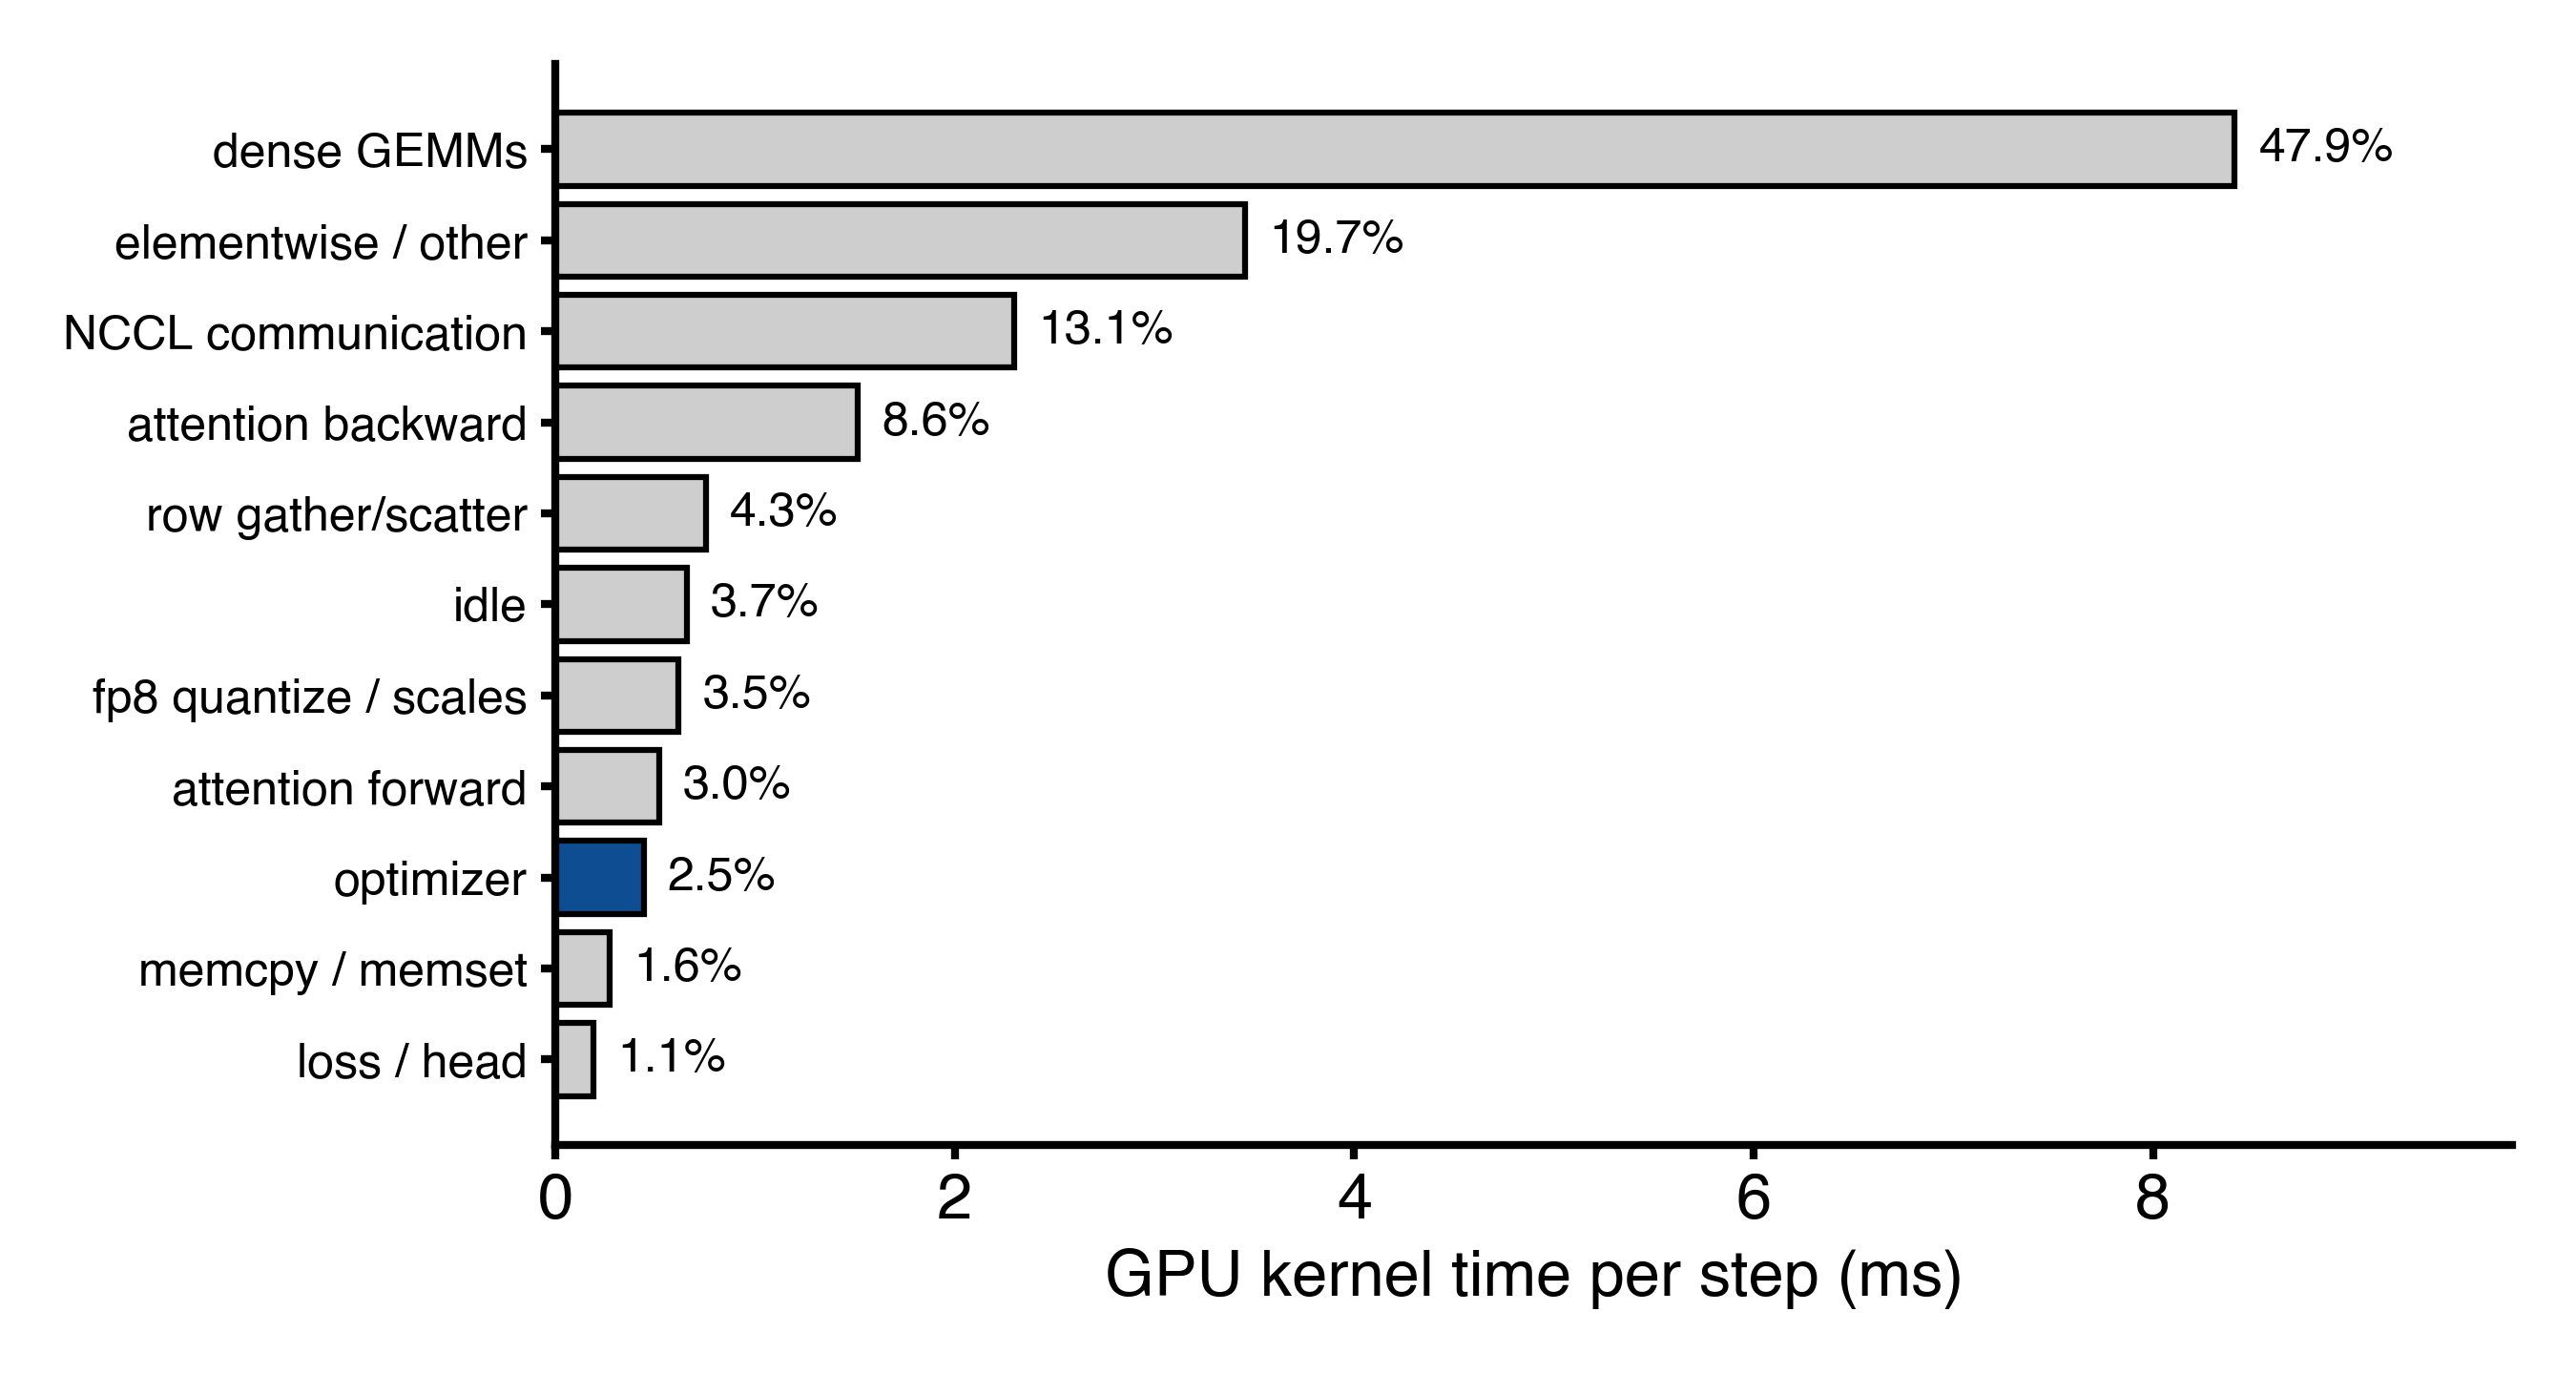
\includegraphics[width=0.85\linewidth]{fig_profile.png}
\caption{GPU kernel time per step in the profiled window (20 steps, the trace of rank 0, one of the eight GPU processes), with each category's share of the $17.55$\,ms step window. The optimizer is highlighted, and the idle row is time with no kernel running. Categories run on overlapping streams, so shares can sum to more than 100\%.}\label{fig:profile}
\end{figure}

\paragraph{Q2: kernel speed and accuracy.} Table~\ref{tab:bench} and Figure~\ref{fig:bench} show the microbenchmark results. The $1.30\times$ speedup compares the matrix sequences only (the six maps), with the record's sequence re-implemented call by call for the comparison. The $1.08\times$ speedup compares the whole update of the group as the trainer runs it, which also includes the momentum computation, the normalization and the weight update. Both are timed as CUDA-graph replays. The error of the kernel relative to the exact update is similar to the record's. For the square and small groups the Gram matrix is not smaller than $X$, and the same change is slower ($0.79\times$ and $0.84\times$ on the full update). We therefore switched only the MLP group. Peak GPU memory is unchanged at $48{,}413$\,MiB.

\begin{table}[!htbp]\centering\small
\begin{tabular}{lrrrrr}\toprule
 & record (ms) & Gram-space (ms) & speedup & record err. & Gram-space err.\\\midrule
matrix sequence & 0.396 & 0.304 & $1.30\times$ & 0.77\% & 0.69\%\\
full update & 0.510 & 0.473 & $1.08\times$ & -- & --\\\bottomrule
\end{tabular}
\caption{MLP group ($3\times2816\times768$), one H100, 300 repetitions (medians). Speedup is the record's time divided by the Gram-space time. Error is relative Frobenius distance from the exact update.}\label{tab:bench}
\end{table}

\begin{figure}[!htb]\centering
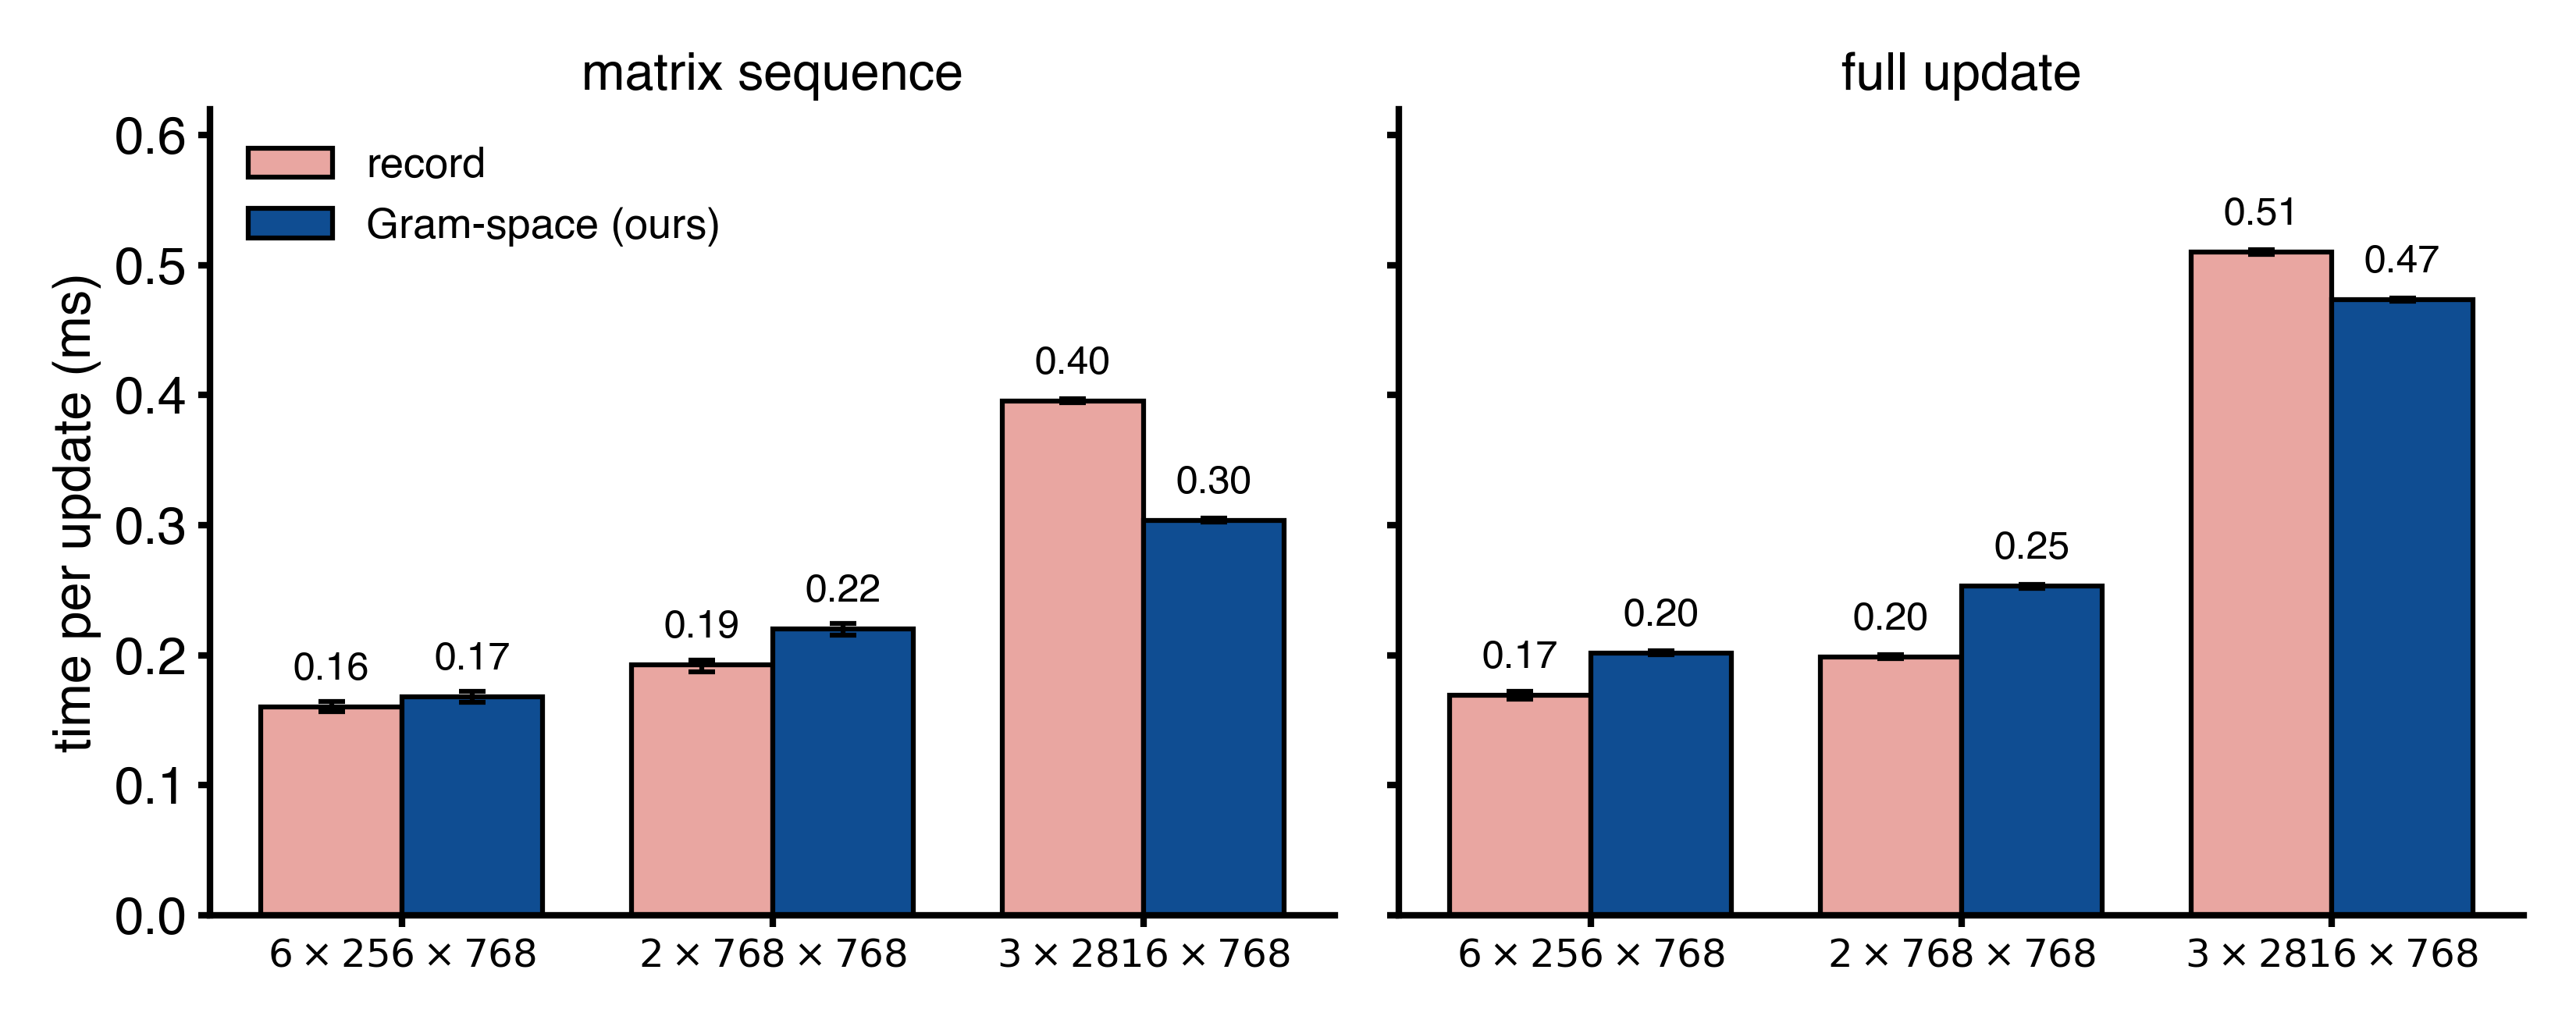
\includegraphics[width=0.95\linewidth]{fig_bench.png}
\caption{Microbenchmark of each weight group's update on one H100 (300 repetitions; bars are medians, whiskers the 10th--90th percentiles). The Gram-space order is faster only for the tall MLP group.}\label{fig:bench}
\end{figure}

\paragraph{Q3: end-to-end time.} Table~\ref{tab:e2e} and Figure~\ref{fig:loop} give the end-to-end comparison. In whole-run training time, the five pairs (seeds 1--3, 6 and 7) give a mean saving of $0.050$\,s (s.e.\ $0.035$, $n=5$, $t=1.4$), which is not significant. In two of the five pairs the kernel was slower in whole-run time: by $0.004$\,s in seed 3 ($40.535$ against $40.531$\,s) and by $0.037$\,s in seed 6 ($40.485$ against $40.448$\,s), where its first step took $259$\,ms and the record's took $158$\,ms. The step loop is more repeatable than the whole-run time. In the step loop the kernel is faster in all five pairs (Figure~\ref{fig:paired}). It saves $0.065\pm0.005$\,ms per step (mean $\pm$ s.e., $n=5$ pairs; $t=13.3$, $p<0.001$), which is $0.077$\,s per run, or $0.2\%$. The ablation saves $0.218\pm0.010$\,ms per step (mean $\pm$ s.e., $n=4$ pairs: seeds 1--3 and 6), which is $0.26$\,s per run. This is our estimate of the upper bound on the saving from a faster implementation of the maps. The kernel's result is consistent with that of Amsel et al.~\cite{polar}.

\begin{table}[!htbp]\centering\small
\begin{tabular}{lrrr}\toprule
 & train time (s), $n=4$ & step loop (s), $n=3$ & final val loss, $n=4$\\\midrule
record & $40.591\pm0.065$ & $40.014\pm0.016$ & $3.27609\pm0.00066$\\
\texttt{gram222s} (Gram-space) & $40.511\pm0.018$ & $39.933\pm0.004$ & $3.27553\pm0.00074$\\
no matrix work (ablation) & $40.320\pm0.041$ & $39.751\pm0.015$ & $3.45510\pm0.00610$\\\bottomrule
\end{tabular}
\caption{Full runs, 1194 steps, mean $\pm$ s.d.\ across seeds, unpaired ($n=4$: seeds 1--4; $n=3$: seeds 1--3). Train time is the whole-run training time, and step loop is the time of the 1193 timed steps. Seeds 1--3 of every arm and seed 4 of the record ran on the first node; seed 4 of the other two arms ran on another node. The last row is the ablation, whose loss does not reach the target.}\label{tab:e2e}
\end{table}

\begin{figure}[!htb]\centering
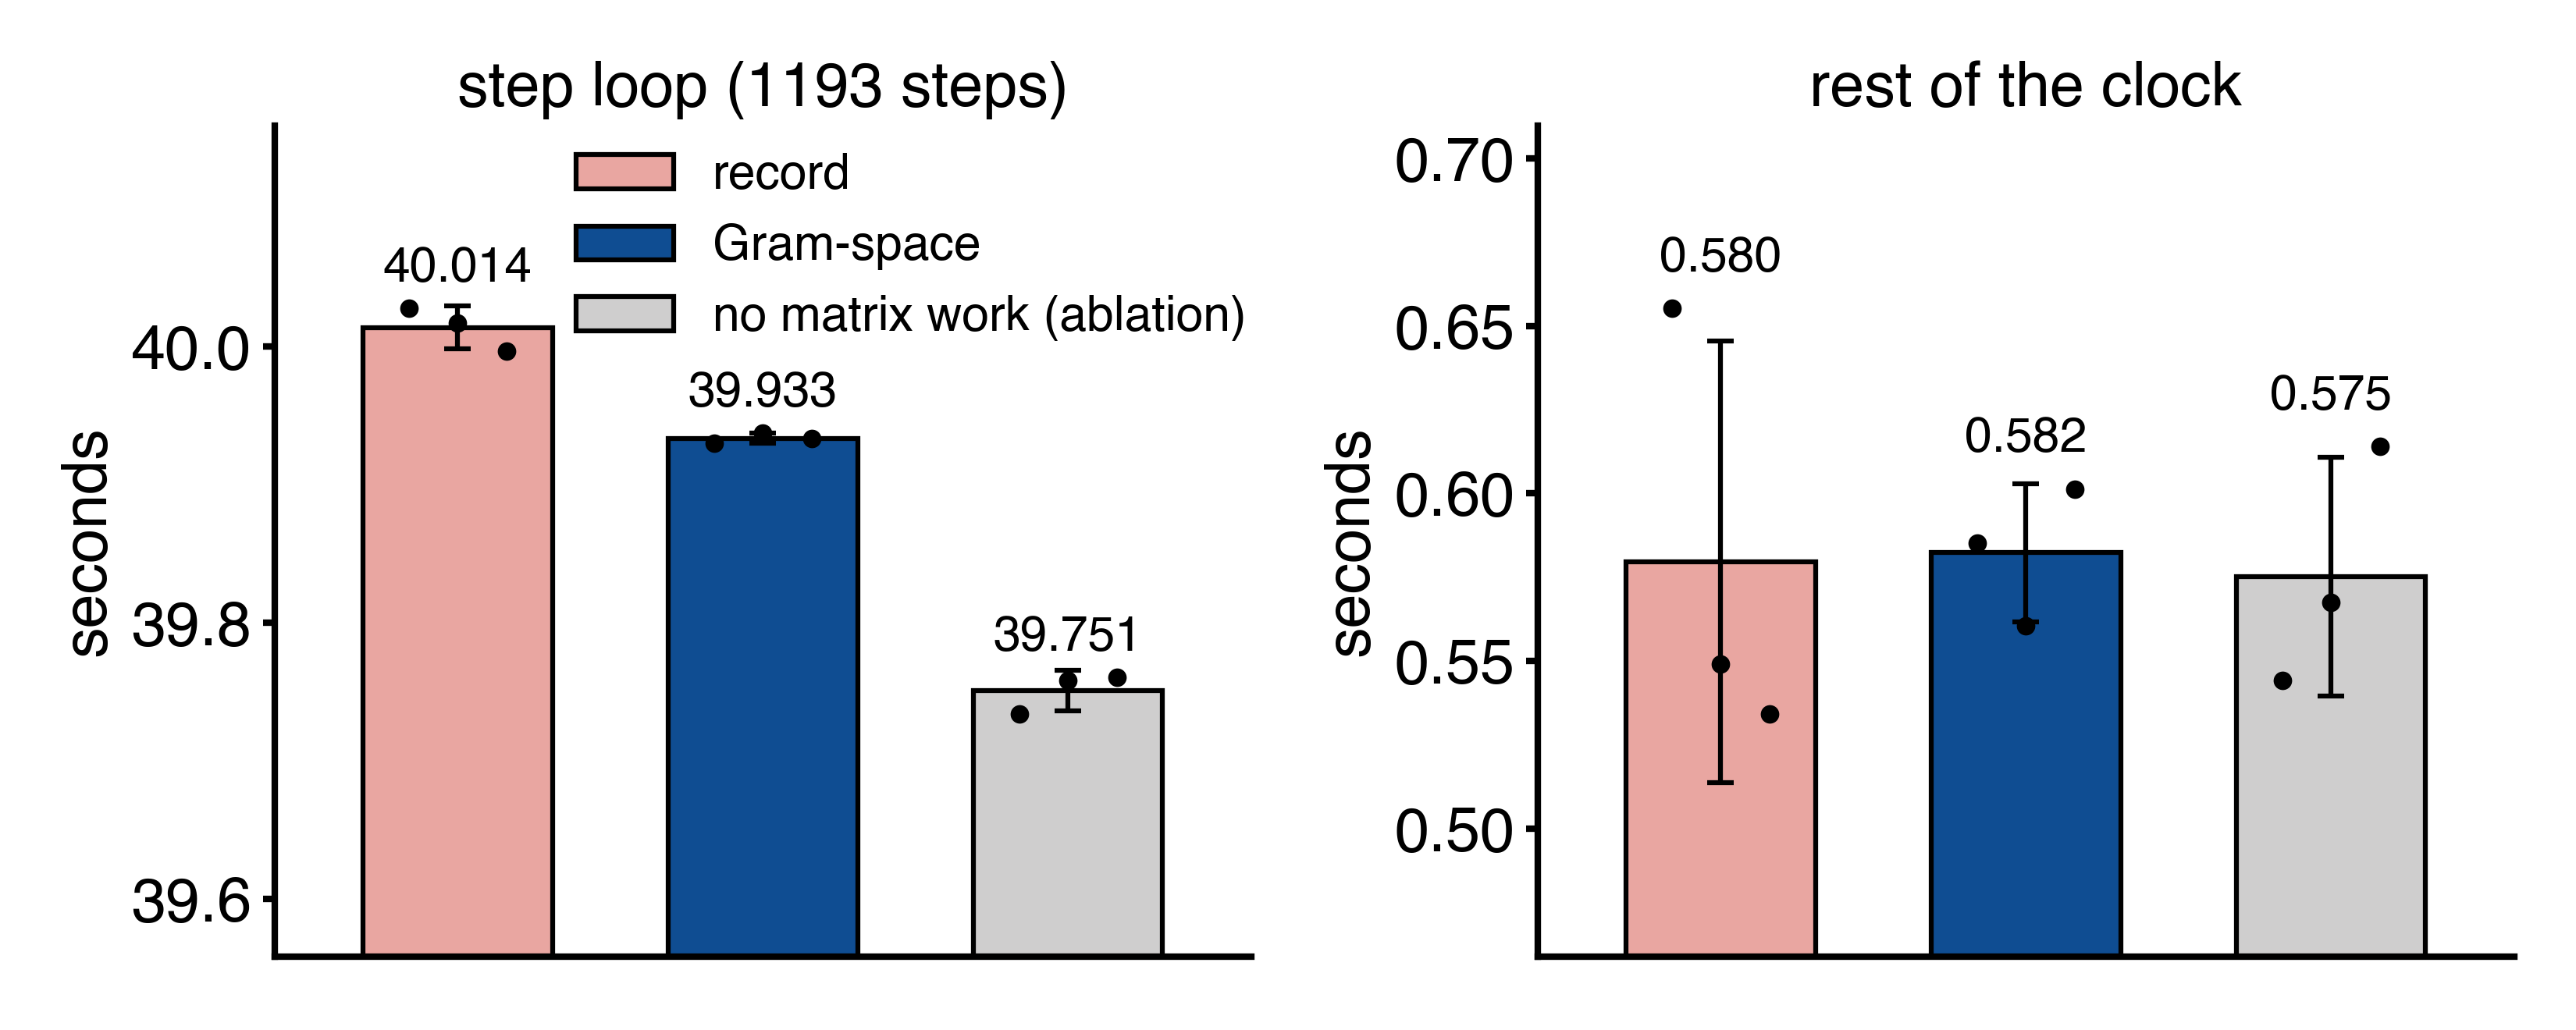
\includegraphics[width=0.95\linewidth]{fig_steploop.png}
\caption{Each run's clock split into the 1193 timed steps (left) and the remainder (right); points are seeds 1--3, bars and whiskers are mean $\pm$ s.d.\ ($n=3$ per arm). The arms separate in the step loop. Across the nine runs the remainder ranges from $0.534$ to $0.655$\,s, a spread that is larger than the kernel's effect.}\label{fig:loop}
\end{figure}

\begin{figure}[!htb]\centering
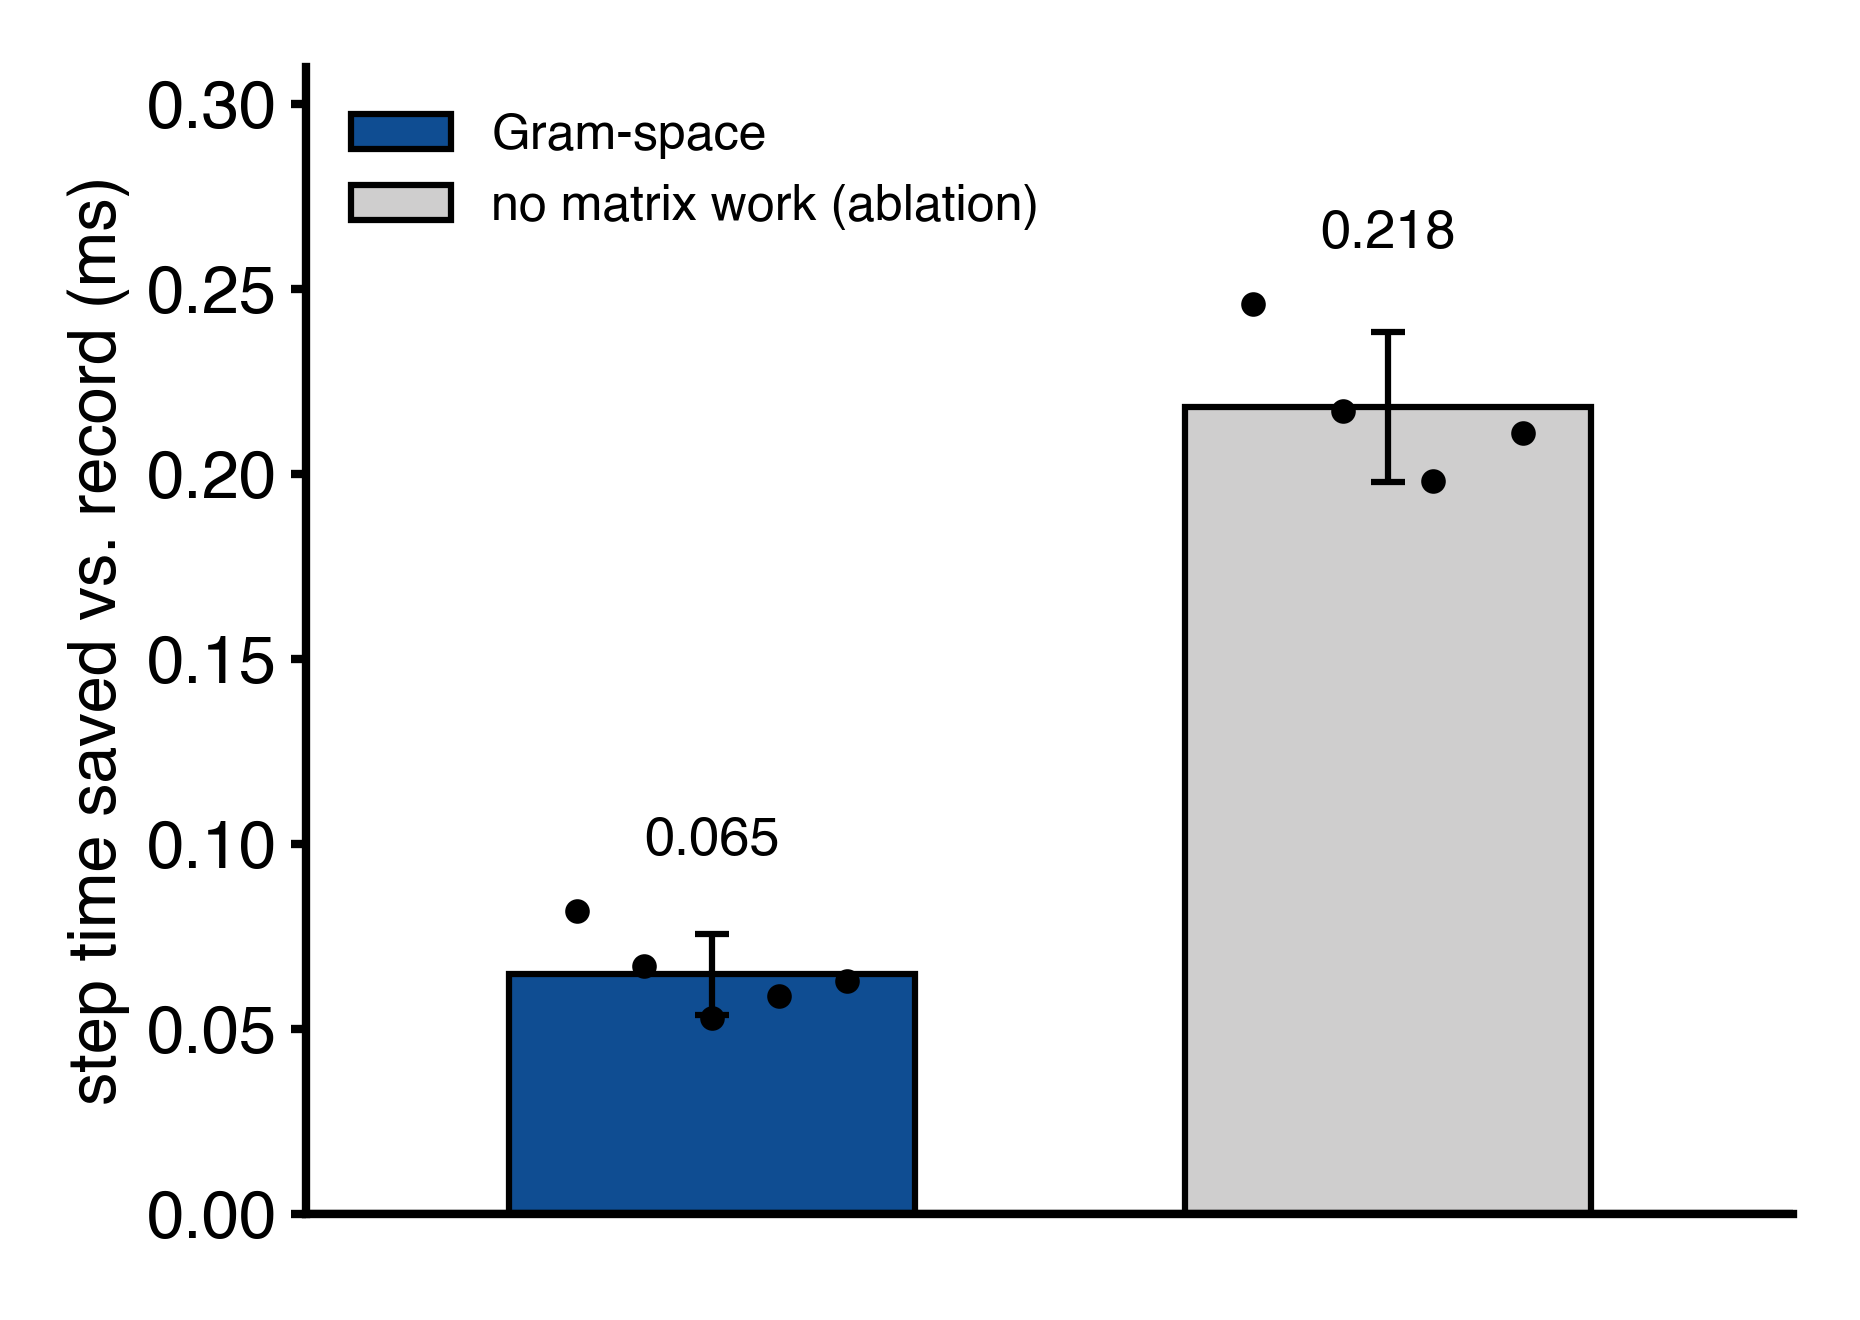
\includegraphics[width=0.5\linewidth]{fig_paired.png}
\caption{Paired difference in mean step time against the record at the same seed (points; bars and whiskers are mean $\pm$ s.d.; $n=5$ pairs for the kernel and $n=4$ for the ablation). Seeds 1--3 ran on the first node with the record first; seeds 6 and 7 ran on a second node with the order swapped between seeds.}\label{fig:paired}
\end{figure}

\paragraph{Q3: validation loss.} Final validation loss is not worse with the kernel: $3.27585\pm0.00080$ against $3.27641\pm0.00073$ (mean $\pm$ s.d., $n=6$ seeds each: 1--4, 6 and 7). The paired difference over these six seeds is $-0.00056$, which is small compared with the margin of about $0.004$ below the target. In the seed-5 curve runs the kernel ended $0.0011$ higher ($3.274384$ against $3.273281$). Every record and kernel run reaches the $3.28$ target, and the validation curves of the two arms, shown for one seed each in Figure~\ref{fig:curve}, differ by at most $0.04$ at intermediate steps and by $0.001$ at the end.

\begin{figure}[!htb]\centering
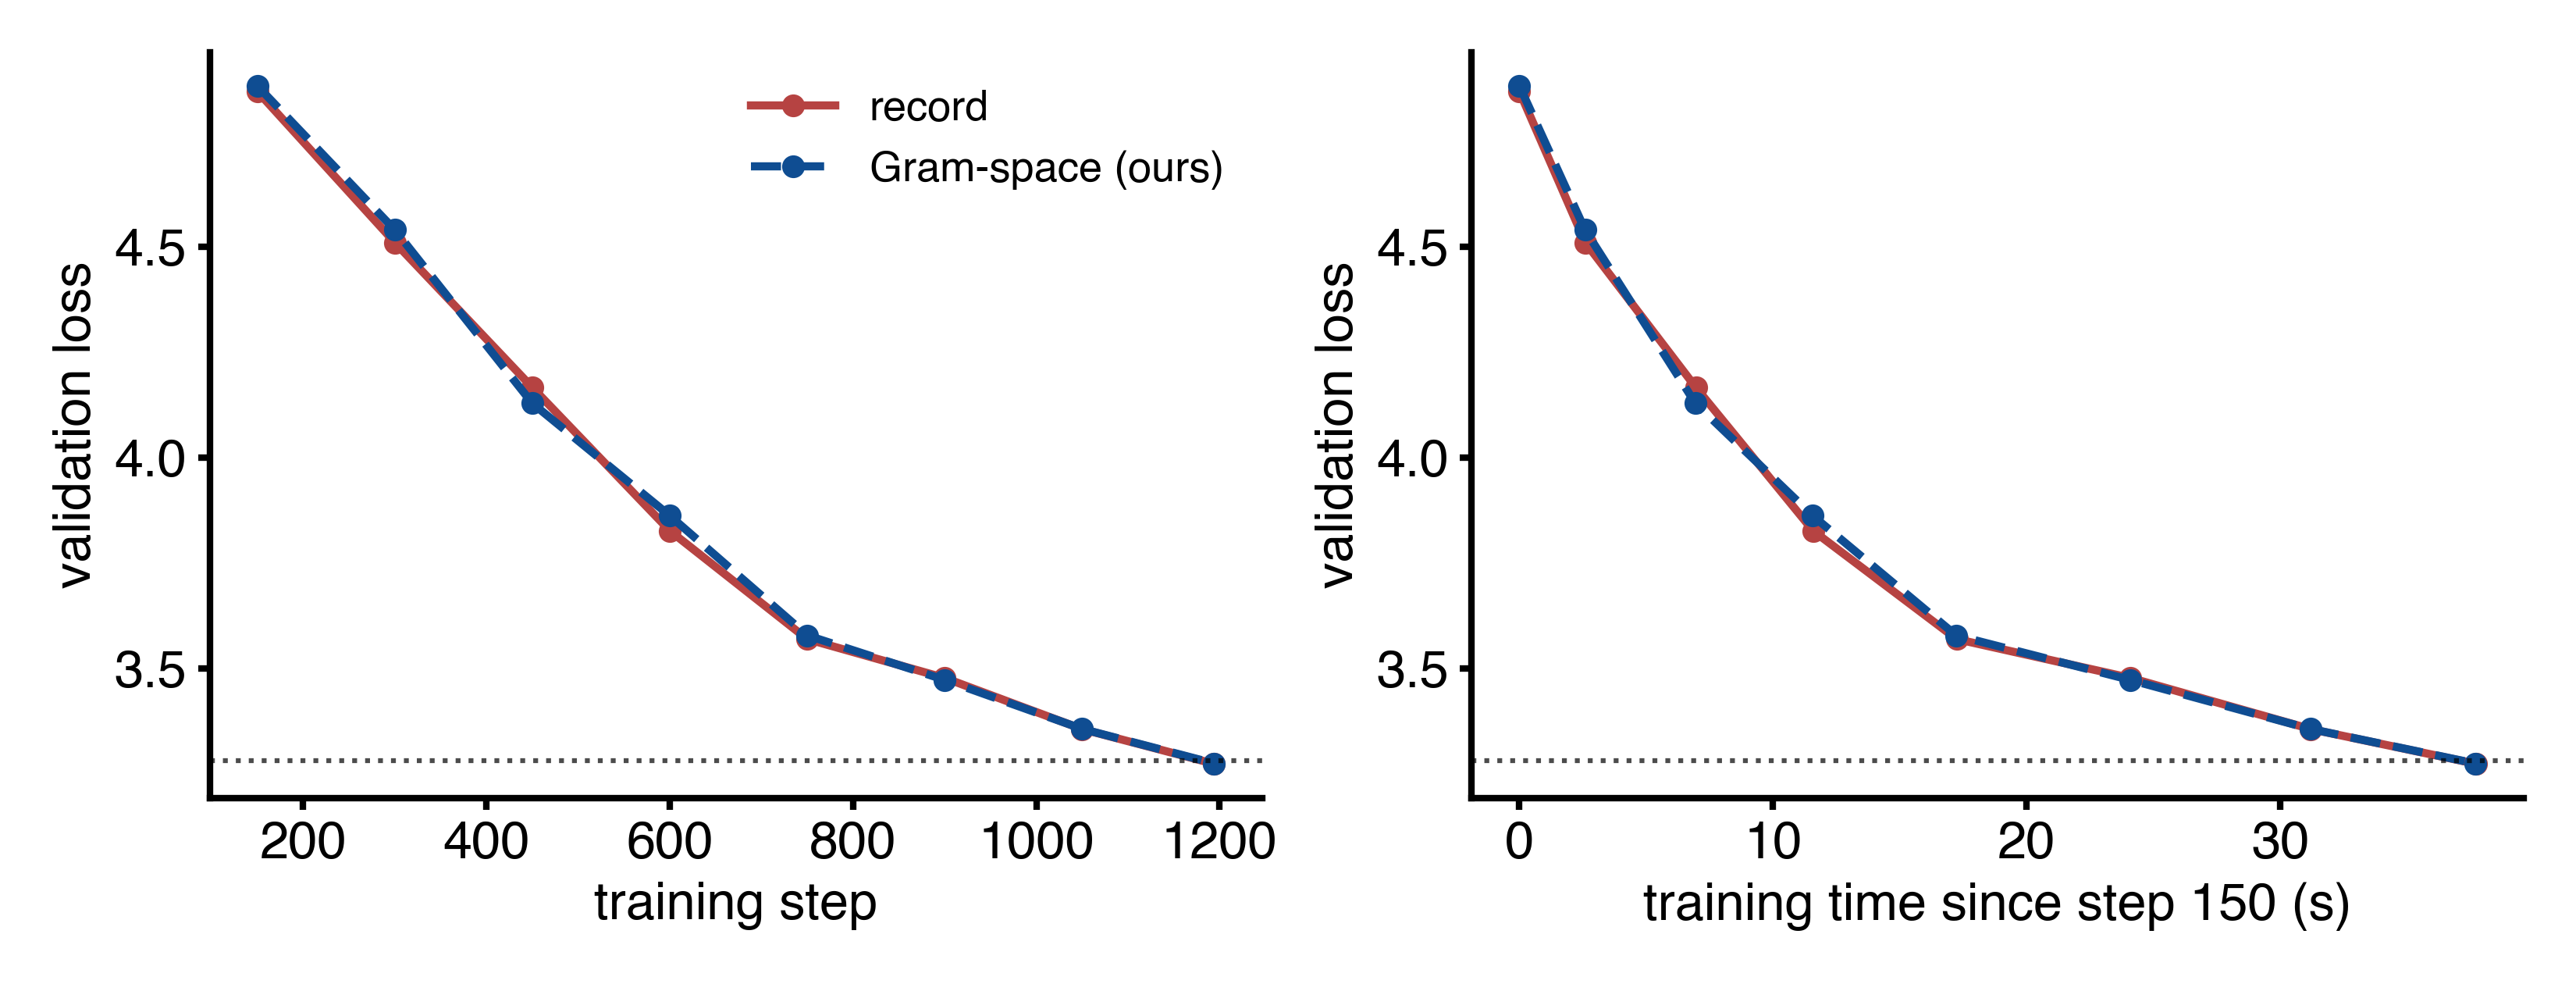
\includegraphics[width=0.95\linewidth]{fig_curve.png}
\caption{Validation loss during training (seed 5, validated every 150 steps; dotted line: the 3.28 target). Left: against training step. Right: against training time measured from the first validation, because a curve run's clock also carries the cost of the extra validations.}\label{fig:curve}
\end{figure}

\section{Interpretation of the small gain}\label{sec:interp}
\paragraph{Saving by stage.} Table~\ref{tab:stage} splits the step time by schedule stage. The matrix work per step is the same in every stage, because the weight matrices do not change size, but the measured saving differs between stages. In the paired runs the ablation saves $0.167$\,ms per step in stage 0, where a step takes $16.9$\,ms, and $0.212$ and $0.264$\,ms in stages 1 and 2, where a step takes $30.7$ and $46.6$\,ms. The kernel saves $0.040$, $0.070$ and $0.084$\,ms in the same stages. Stages 3 and 4 have 67 and 20 steps per run, and their savings have an s.e.\ of $0.02$ to $0.04$\,ms, so they do not separate from the other stages. The saving varies although the removed work is constant, which suggests that the time recovered depends on the rest of the step. The table does not identify the cause.

\begin{table}[!htbp]\centering\small
\begin{tabular}{lrrrrrr}\toprule
 & all & stage 0 & stage 1 & stage 2 & stage 3 & stage 4\\\midrule
steps counted & 1193 & 319 & 361 & 426 & 67 & 20\\
record (ms) & 33.544 & 16.937 & 30.653 & 46.590 & 46.570 & 29.065\\
\texttt{gram222s} (ms) & 33.445 & 16.891 & 30.525 & 46.470 & 46.501 & 29.038\\
no matrix work (ms) & 33.294 & 16.767 & 30.383 & 46.292 & 46.336 & 28.873\\\midrule
paired saving, \texttt{gram222s} (ms) & $0.065$ & $0.040$ & $0.070$ & $0.084$ & $0.042$ & $0.006$\\
\quad s.e., $n=5$ & $0.005$ & $0.003$ & $0.013$ & $0.006$ & $0.021$ & $0.026$\\
paired saving, no matrix work (ms) & $0.218$ & $0.167$ & $0.212$ & $0.264$ & $0.195$ & $0.202$\\
\quad s.e., $n=4$ & $0.010$ & $0.004$ & $0.020$ & $0.015$ & $0.024$ & $0.040$\\\bottomrule
\end{tabular}
\caption{Mean step time by schedule stage. Upper rows: mean over the four runs of each arm (seeds 1--4), unpaired. Lower rows: mean and s.e.\ of the same-seed, same-session saving relative to the record, computed as the record minus the arm, so that positive values mean the arm is faster (seeds 1--3, 6 and 7 for the kernel; seeds 1--3 and 6 for the ablation). Differences between the upper rows are larger than the paired savings ($0.099$ against $0.065$\,ms overall for the kernel) because seed 4 of the two non-record arms ran on another node.}\label{tab:stage}
\end{table}

\paragraph{Overlap with other GPU work.} The microbenchmark measures $0.593$\,ms of matrix work per step, and removing that work in training shortens a step by $0.218$\,ms. The critical path of a step is the chain of operations that determines when the step ends, and work that runs at the same time as that chain does not lengthen the step. One reading of the two numbers is that about $60\%$ of the matrix work overlaps other activity on the GPU and is not on the critical path. This is an inference from comparing an isolated benchmark with an in-training ablation, and we did not measure the overlap directly. The microbenchmark runs on one GPU with synthetic inputs, so the two numbers are not directly comparable. For example, the kernel's saving in training ($0.065$\,ms per step) is larger than its saving in the microbenchmark's full update ($0.037$\,ms).

\paragraph{Cost per GPU kernel.} The Gram-space order reduces the arithmetic of the MLP group from $104$ to $71$\,GFLOP per step (one GFLOP is $10^9$ floating-point operations), but the time falls by a smaller proportion. In the microbenchmark's per-operation timings, a product with the $2816\times768$ matrices takes $0.022$--$0.030$\,ms and a $768\times768$ product takes $0.014$--$0.016$\,ms. A small product therefore has $27\%$ of the arithmetic of a large product and about $60\%$ of its time. These timings suggest that at these sizes a GPU kernel has a fixed cost that does not shrink with its arithmetic, such as the cost of launching it. This statement rests on the benchmark's per-operation timings, and launch cost was not measured separately. For each pair of maps, the change replaces six GPU kernels on the large matrices (two Gram computations, two products and two additions) with two, and adds three small products.

\paragraph{Related measurements in open speedrun submissions.} Two open pull requests to the speedrun repository, both stacked on other open submissions, are consistent with these results. One reduces the sequence from six maps to four and reports a saving of $0.19$\,s at equal loss\footnote{\url{https://github.com/KellerJordan/modded-nanogpt/pull/393}}. This is of the same order as our $0.26$\,s estimate for removing all six maps, although the trainers differ. The other reports a saving of $0.35$\,s from host-side fixes at the start and end of the clock (end-of-run time $370$\,ms to about $30$\,ms, start $170$\,ms to $44$\,ms)\footnote{\url{https://github.com/KellerJordan/modded-nanogpt/pull/404}}. That time corresponds to the remainder outside the step loop in our runs, whose variation is larger than the kernel's effect, and the reported saving is larger than our estimate of the upper bound for the optimizer's matrix work. These are the authors' own measurements, and we did not reproduce them.

\FloatBarrier
\section{Limitations}
The end-to-end runs are few (five pairs for the kernel and four for the ablation, over two nodes). In four of the five kernel pairs and in all four ablation pairs the record ran before the other arm, and one of those record runs was the first run on its node. The upper bound is an estimate from four pairs and covers the matrix work of the maps only. Step latencies are read on the host CPU without a GPU synchronization, that is, without waiting for the GPU to finish its queued work, so only means over many steps are used. The profile covers one early window. The per-operation timings come from one GPU, and the upper rows of Table~\ref{tab:stage} and one ablation pair include runs from a second node. Figure~\ref{fig:curve} shows validation loss only, for one seed per arm. Runs that also log training loss, over three seeds per arm, were submitted but had not finished when this version was written. The time outside the step loop is about $0.15$\,s before the end of the first step and $0.39$\,s after the last step, and we did not try to reduce it. The conclusions are specific to this model, trainer and hardware.

\section{Reproducibility}
A summary of the main result was posted to the speedrun repository's discussions\footnote{\url{https://github.com/KellerJordan/modded-nanogpt/discussions/405}}. Code, job scripts, raw logs and the scripts that regenerate every figure and the values in the tables are in the repository \url{https://github.com/ethantsliu/182-project}, in the directories \path{182/results/}, \path{182/optim-kernel/} and \path{182/paper/}. The kernel is enabled with the environment setting \path{ANVIL_KERNEL=gram222s} and the ablation with \path{ANVIL_ABLATE=skip_matrix}. With no flag set, the trainer is the record. Checkpoints will be added with V2. Figure styling follows the conventions of the \texttt{figures4papers} repository by Chen Liu (\url{https://github.com/ChenLiu-1996/figures4papers}).

\begin{thebibliography}{15}\small
\bibitem{shampoo} Vineet Gupta, Tomer Koren, Yoram Singer. Shampoo: Preconditioned Stochastic Tensor Optimization. Proceedings of the 35th International Conference on Machine Learning (ICML), PMLR 80, 2018. \url{https://proceedings.mlr.press/v80/gupta18a.html}
\bibitem{anil} Rohan Anil, Vineet Gupta, Tomer Koren, Kevin Regan, Yoram Singer. Scalable Second Order Optimization for Deep Learning. arXiv:2002.09018, 2020.
\bibitem{soap} Nikhil Vyas, Depen Morwani, Rosie Zhao, et al. SOAP: Improving and Stabilizing Shampoo using Adam. arXiv:2409.11321, 2024.
\bibitem{muonblog} Keller Jordan, Yuchen Jin, Vlado Boza, et al. Muon: An optimizer for hidden layers in neural networks. Blog post, 2024. \url{https://kellerjordan.github.io/posts/muon/}
\bibitem{muon} Jingyuan Liu, Jianlin Su, Xingcheng Yao, et al. Muon is Scalable for LLM Training. arXiv:2502.16982, 2025.
\bibitem{polar} Noah Amsel, David Persson, Christopher Musco, Robert M. Gower. The Polar Express: Optimal Matrix Sign Methods and Their Application to the Muon Algorithm. ICLR 2026; arXiv:2505.16932, 2025.
\bibitem{gramns} Jack Zhang, Noah Amsel, Berlin Chen, Tri Dao. Gram Newton--Schulz: A Fast, Hardware-Aware Newton--Schulz Algorithm for Muon. Blog post and code, 2026. \url{https://tridao.me/blog/2026/gram-newton-schulz/}
\bibitem{cachemuon} Bishnu Dev, Sushil Bohara, Martin Tak\'a\v{c}, Samuel Horv\'ath. CacheMuon: Using Temporal Preconditioning To Approximate Polar Factor. arXiv:2606.16371, 2026.
\bibitem{transportmuon} Ethan Smith. Transport Muon: Beating Muon in Speed and Performance in 1 Newton Step. Blog post and code, 28 April 2026. \url{https://ethansmith2000.substack.com/p/transport-muon-beating-muon-in-speed}
\bibitem{fantastic} Kaiyue Wen, David Hall, Tengyu Ma, Percy Liang. Fantastic Pretraining Optimizers and Where to Find Them. ICLR 2026; arXiv:2509.02046, 2025.
\bibitem{fp8} Paulius Micikevicius, Dusan Stosic, Neil Burgess, et al. FP8 Formats for Deep Learning. arXiv:2209.05433, 2022.
\bibitem{triton} Philippe Tillet, H. T. Kung, David Cox. Triton: An Intermediate Language and Compiler for Tiled Neural Network Computations. MAPL 2019 (workshop at PLDI 2019), 2019.
\bibitem{fa3} Jay Shah, Ganesh Bikshandi, Ying Zhang, Vijay Thakkar, Pradeep Ramani, Tri Dao. FlashAttention-3: Fast and Accurate Attention with Asynchrony and Low-precision. Advances in Neural Information Processing Systems 37 (NeurIPS 2024), 2024.
\bibitem{speedrun} Keller Jordan, Jeremy Bernstein, Brendan Rappazzo, et al. modded-nanogpt: Speedrunning the NanoGPT baseline. Code repository, 2024. \url{https://github.com/KellerJordan/modded-nanogpt}
\bibitem{anvil2} Deven Pietrzak. New Record: 0.665 minutes (39.9 seconds): ANVIL2, Sampled-softmax, New Embedding Table, Full-stack fp8. Pull request 360, KellerJordan/modded-nanogpt, merged 28 September 2026. \url{https://github.com/KellerJordan/modded-nanogpt/pull/360}. Write-up: Training NanoGPT in 39.9 Seconds, 27 September 2026. \url{https://hyperstition.cc/training-nanogpt-in-39-9-seconds}
\end{thebibliography}

\appendix
\section{Use of generative AI}
We used ChatGPT to brainstorm and refine the research question and to help draft the proposal. We used Grok and Claude to help with the initial baseline reproduction. We used Claude Code to implement the alternative kernel, its tests and the benchmark, to write the job scripts and run the experiments on rented GPUs, to parse logs into the tables and figures, and to draft this report. The authors reviewed the code, the results and the text. \emph{[Team: revise so this matches what each of us actually did.]}

\section{Other runs}
The runs in this appendix are reproductions of other people's speedrun submissions and small tuning checks on one of them. They are not part of the study in the main text, and the times are for our node type. Source tables are in \texttt{182/results/README.md}.

\paragraph{Upstream GPU-only tree (pull request 397).} Two runs both logged $30.719$\,s, with validation losses of $3.27672$ and $3.27712$ ($n=2$, random seeds). Two runs do not give a spread.

\paragraph{Upstream CPU n-gram tree (pull request 381).} Seventeen runs across five jobs reached the target in a mean of $10.170$\,s (s.d.\ $0.321$, $n=17$), or $10.000$\,s without the first run of each job ($n=12$). The worst validation loss was $3.2778$. We do not use this tree as the baseline because it is an open, unmerged submission that uses the host CPUs for retrieval during training, and a maintainer has said that rules on CPU use are still to be set. The main text uses the merged record.

\paragraph{Scheduled-step trim on the CPU n-gram tree (675 to 668 steps).} In eight interleaved same-seed pairs, the 668-step runs were $0.131$\,s faster (s.e.\ $0.039$, $n=8$, $p=0.013$). Without the first pair of each job, which ran right after the warm-up run, the difference is $0.077$\,s (s.e.\ $0.024$, $n=6$). The trim raised the validation loss by $0.00181$ (s.e.\ $0.00016$, $n=8$ pairs). All eleven 668-step runs were at or under $3.28$, with a mean of $3.27688$ (s.d.\ $0.00146$, $n=11$), and one run logged $3.2800$.

\paragraph{\texttt{TABLE\_VOTE} option on the CPU n-gram tree.} Three same-seed pairs showed no effect of the option. The runs with the option were $0.064$\,s faster (s.e.\ $0.127$, $n=3$, $p=0.66$), and the loss difference, computed as the run with the option minus the run without it, was $-0.00003$ (s.e.\ $0.00047$, $n=3$).
\end{document}
